\chapter{Boosting shortest path multiplicity}
\label{ch:distance}

\section{The redundancy of shortest paths}

The small-world property, met back in the introduction, promises that any two
nodes of a real network are joined by a \emph{short} path --- only a few hops
apart. It says nothing, though, about how \emph{many} short paths there are.
That count turns out to matter a great deal. If the only shortest route between
two nodes runs through a single chain of intermediaries, the connection is
fragile: cut one link and the shortest route is gone. If instead there are
several shortest routes side by side, the connection is robust, and whatever
flows between the two nodes --- a message, a signal, a delay --- can travel along
all of them at once. The quantity that captures this is the \emph{shortest path
multiplicity}: the number of distinct shortest routes between a pair of nodes. A
simple picture: if two friends can each be reached from you in two handshakes,
but by two completely different chains of acquaintances, the multiplicity of that
connection is two. In real networks this multiplicity is conspicuously high.

And it is not an isolated fact. \citet{deng2026} found that, across many real
networks, the abundance of multiple shortest paths is strongly correlated with
\emph{community structure} --- the very groupings of the previous chapter ---
more strongly than with any other standard measure. Two networks of the same size
and the same degree distribution can differ widely in their path multiplicity,
and the difference tracks how community-rich they are. A correlation like that
begs for an explanation. Does community structure somehow \emph{cause} paths to
multiply, or do both spring from a common deeper source? The previous chapter
hands us the obvious suspect: local growth rules, which we saw conjure
communities out of nothing but locality. This chapter, following
\citet{vazquezpaths2026}, completes the case by showing that those same local
rules also \emph{boost} the multiplicity of shortest paths --- so that the
striking link between paths and communities is not one causing the other, but the
shared shadow cast by the rule that grew the network.

The mechanism is easy to picture once named. Local rules build short
\emph{cycles} --- closed loops --- as a matter of course: a triangle whenever a
friend introduces a friend, a square whenever a gene is copied. And a cycle is
exactly a structure that offers more than one way around. In a network with no
loops at all --- a \emph{tree} --- there is precisely one route between any two
nodes; the more loops a network carries, the more alternative shortest routes it
affords. Path multiplicity is simply what local rules leave behind when they
close loops.

\section{Defining the multiplicity}

We need only one quantity. Write $\mu_{ij}(G)$ for the number of distinct
shortest paths between nodes $i$ and $j$ in a network $G$ --- counting every route
that ties for the minimum number of hops. Averaging this over all pairs of nodes,
and over many networks grown the same way, gives the \emph{average shortest path
multiplicity} $\langle\mu\rangle$, the single number we will follow as the
network grows to size $n$. A tree, with its unique routes, has $\langle\mu\rangle
= 1$ exactly; anything above one measures the redundancy that loops provide. The
whole chapter is about one question: how fast does $\langle\mu\rangle$ rise as the
network gets bigger, and does that rate betray whether the network was grown by a
local rule?

Three growth rules will do all the work, and we have met them all before. The
\emph{local-search} model $LS(n,m)$ of Chapter~\ref{ch:search}: a newcomer starts
at a random node, takes an $m$-step walk, and links to every node it visits. The
\emph{duplication--split} model $DS(n,q)$ of Chapter~\ref{ch:projects}: with
probability $q$ a randomly chosen node is copied along with all its links,
otherwise one of its links is split in two. And the \emph{bubble} model
$BB(n,L)$ of the previous chapter: a chain of $L$ new nodes is attached by its two
ends to the two ends of an existing link, closing a fresh cycle of length $L+2$.
Against these we set the Barab\'asi--Albert model $BA(n,m)$, which is
\emph{not} local: its newcomers weigh the whole network.

\section{The baseline: random networks}

To judge what counts as ``boosted,'' we first need the expectation in the
\emph{absence} of any local structure. The natural reference is a random network,
and here we can do better than simulate --- we can calculate. The answer is
remarkably simple, and it turns on a single property of the degree distribution:
the \emph{average excess degree}
\begin{equation}
  c_2 = \frac{\langle k(k-1)\rangle}{\langle k\rangle},
  \label{eq:path-c2}
\end{equation}
which is the average number of \emph{further} links you find when you arrive at a
node by following one of its links --- its degree, less the link you came in on.
It is the natural branching factor of a network: from where you stand, $c_2$ is
how many ways the path onward can continue.

\begin{calculation}{how many shortest paths a random network has}
Take a random network in which the chance that two nodes are linked depends only
on their degrees. Fix two nodes and count the paths of length $d$ between them.
There are about $n^{d-1}$ candidate paths --- that many ways to pick the ordered
intermediaries --- and each survives only if all $d$ of its links happen to be
present. Arriving at a node along a link, the onward branching is $c_2$ on
average, so the expected number of realized paths of length $d$ is
\begin{equation}
  \langle M_d\rangle \approx c_1 c_2^{\,d-D-1},
  \label{eq:path-Md}
\end{equation}
where $c_1=\langle k\rangle$ and $D = \ln n/\ln c_2$ is the typical distance.
The shortest paths are the ones at the first $d$ where any path exists at all, so
we must weight $\langle M_d\rangle$ by the probability $F_{d-1}$ that nothing
shorter exists. Treating the paths as independent, $F_d \approx \exp(-\langle
M_d\rangle)$, and
\begin{equation}
  \langle\mu\rangle \approx \sum_d \langle M_d\rangle\, F_{d-1}.
  \label{eq:path-mu-sum}
\end{equation}
The summand rises geometrically in $d$ and is then cut off super-exponentially by
$F_{d-1}$, so it peaks sharply one hop beyond $D$. Evaluating it there leaves
\begin{equation}
  \langle\mu\rangle \approx \frac{c_2}{e},
  \label{eq:path-mf}
\end{equation}
the factor $e$ arriving from the value of $x e^{-x}$ at its peak. The whole
distribution of degrees enters through the single number $c_2$.
\end{calculation}

Equation~\eqref{eq:path-mf} is the baseline, and it is worth pausing on how much
it explains. The multiplicity of a random network is simply its branching factor,
divided by $e$. Everything then hinges on how $c_2$ behaves as the network grows,
and for a scale-free network, $p(k)\sim k^{-\gamma}$, that depends entirely on the
exponent $\gamma$. Since $c_2$ involves $\langle k^2\rangle$, it is controlled by
the hubs, and the largest degree in a network of $n$ nodes grows like
$k_{\max}\sim n^{1/\gamma}$. Three regimes follow:
\begin{alignat}{2}
  \langle\mu\rangle &= a, &&\qquad \gamma>3,
  \label{eq:path-const}\\
  \langle\mu\rangle &= a + \tfrac{1}{e}\ln n, &&\qquad \gamma=3,
  \label{eq:path-log}\\
  \langle\mu\rangle &= a + b\,n^{\alpha}, \qquad \alpha = \tfrac{3}{\gamma}-1,
    &&\qquad 2<\gamma<3.
  \label{eq:path-power}
\end{alignat}
When $\gamma>3$ the second moment converges, $c_2$ tends to a constant, and the
multiplicity \emph{stops growing altogether}. At $\gamma=3$ the second moment
diverges logarithmically and the multiplicity creeps up like $\ln n$ --- about as
slow as growth gets, since to add a fixed amount you must \emph{multiply} the
size. Below $\gamma=3$ the hubs are heavy enough to drive a genuine power law.
So there is no single random baseline: the bar that a local rule must clear is
set by the degree distribution it happens to produce, and we must compare like
with like.

That is exactly what the simulations do (Figure~\ref{fig:mu-random}). Take a
network grown by a local rule and shuffle its links at random while leaving every
node's degree untouched --- the same configuration-model scramble used as a
control in the previous chapter. The result keeps the degree distribution and
destroys everything else; we mark it with a star. The randomized local-search
network $LS(n,1)^*$ has $\gamma=5$, and its multiplicity duly flattens out. The
randomized $DS(n,1/3)^*$ has $\gamma=3$, and creeps up logarithmically, close to
the predicted slope $1/e$. The randomized $DS(n,2/5)^*$ has $\gamma=5/2$, and
climbs as the predicted $n^{1/5}$. Plotted against $c_2$ rather than $n$, all of
them --- and the Barab\'asi--Albert model with them --- collapse onto the single
mean-field line $c_2/e$.

\begin{figure}[t]
\centering
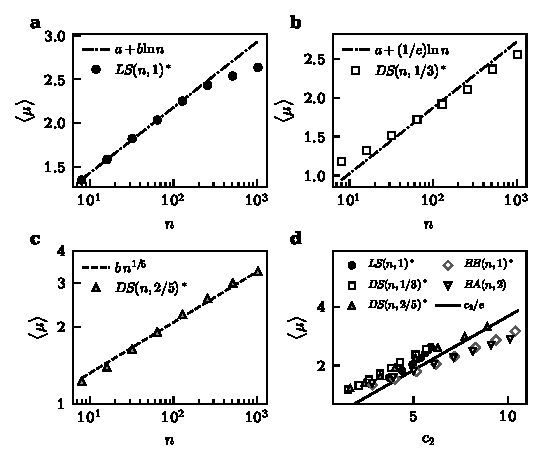
\includegraphics[width=\linewidth]{figs/fig-mu-random.pdf}
\caption{\textbf{The random baseline.} Average shortest path multiplicity
$\langle\mu\rangle$ against network size $n$ for randomized networks (starred),
which keep each node's degree but destroy all local structure. (a) $LS(n,1)^*$,
degree exponent $\gamma=5$: growth stalls, the points falling away from the
fitted logarithm. (b) $DS(n,1/3)^*$, $\gamma=3$: logarithmic, near the predicted
slope $1/e$. (c) $DS(n,2/5)^*$, $\gamma=5/2$: the predicted power law $n^{1/5}$.
(d) All models, including the non-local $BA(n,2)$, plotted against the excess
degree $c_2$ collapse onto the mean-field line $c_2/e$ of
Eq.~\eqref{eq:path-mf}.}
\label{fig:mu-random}
\end{figure}

The Barab\'asi--Albert model deserves its own note, because it is a
\emph{growing} network yet lands squarely on the random baseline. With $m=2$ it
has $\gamma=3$, and its multiplicity creeps up logarithmically, exactly as its
reshuffled cousins do. It has no local structure to lose: its newcomers attach
across the whole graph and never consult a neighborhood. This echoes the previous
chapter, where the very same model failed to develop communities. Lacking
locality, it builds neither the modules nor the redundant paths, and on both
counts it behaves as though its links had been shuffled at random.

\section{Local rules boost the multiplicity}

Now run the same models \emph{without} shuffling, and compare each against its own
starred baseline (Figure~\ref{fig:mu-local}). The multiplicity climbs decisively
faster. It helps to keep a ladder of growth rates in mind: constant, then
logarithmic, then \emph{log-quadratic}, then \emph{exponential} --- each rung
leaving the one below it far behind.

Most local rules --- local search and the bubble model among them --- sit on the
log-quadratic rung,
\begin{equation}
  \langle\mu\rangle = a + b\ln n + c(\ln n)^2,
  \label{eq:path-typeI}
\end{equation}
the extra squared term bending the curve clearly upward. For $LS(n,1)$ this is a
particularly sharp contrast: the unshuffled network grows without limit while the
shuffled one, with the very same degrees, stops growing altogether. Whatever is
doing the work is not in the degree distribution at all.

The duplication--split rule is different, and dramatically so: its multiplicity
grows \emph{exponentially} with size,
\begin{equation}
  \langle\mu\rangle = a\, e^{bn}, \qquad a,b>0.
  \label{eq:path-typeII}
\end{equation}
Exponential growth is a different world from logarithmic. Over the same range of
sizes in which its shuffled counterpart moves from $\langle\mu\rangle\approx1.2$
to $2.6$, the unshuffled $DS(n,1/3)$ runs from $1.3$ to more than $10^5$: by a
thousand nodes, a typical pair of nodes is joined by hundreds of thousands of
equally short routes. Copying, it turns out, is the great multiplier of shortest
paths, and that is what the title of this chapter names.

\begin{figure}[t]
\centering
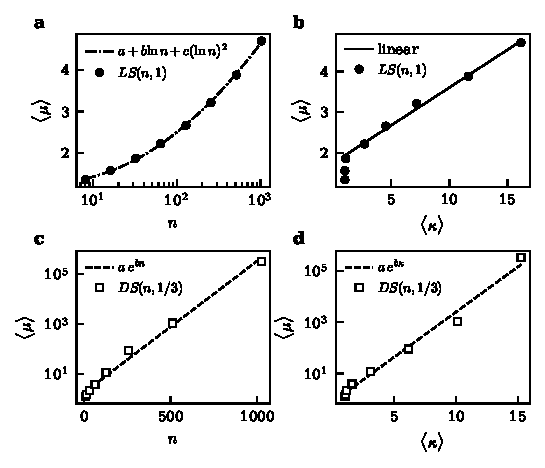
\includegraphics[width=\linewidth]{figs/fig-mu-local.pdf}
\caption{\textbf{Local rules boost the multiplicity.} (a) Local search
$LS(n,1)$ grows log-quadratically, Eq.~\eqref{eq:path-typeI} --- while its
shuffled counterpart, with identical degrees, saturates
(Figure~\ref{fig:mu-random}a). (b) The same data against the inferred number of
communities $\langle\kappa\rangle$: linear. (c) Duplication--split $DS(n,1/3)$
grows exponentially, Eq.~\eqref{eq:path-typeII}; note the linear size axis and
the logarithmic multiplicity axis, and that the vertical scale spans five decades.
(d) Against $\langle\kappa\rangle$: exponential again. Communities are only
detectable beyond the Ramsey size $r_\kappa$, so the leftmost points in (b) and
(d) sit at $\langle\kappa\rangle=1$.}
\label{fig:mu-local}
\end{figure}

\section{Cycles and the boost}

Why should duplication outrun the rest? The answer is in the kind of loop each
rule makes. The triadic-closure rule of the friends chapter closes
\emph{triangles}, loops of length three --- but in a triangle the two nodes
flanking a third are themselves directly linked, so there is still only \emph{one}
shortest route between any pair. A triangle adds cohesion but no extra routes.
Duplication, by contrast, closes \emph{squares}, loops of length four, and a
square is the smallest loop that genuinely offers a choice: its two opposite
corners are two hops apart by \emph{two} different paths, one around each side.
That single observation is the seed of the boost; the box pushes it a little
further, and the takeaway follows.

\begin{figure}[t]
\centering
\begin{adjustbox}{max width=\linewidth}\begin{tikzpicture}[
  nd/.style={circle,draw=black!65,fill=black!4,minimum size=6mm,inner sep=0pt},
  ep/.style={circle,draw=accent!80!black,fill=black!30,minimum size=6mm,inner sep=0pt},
  lnk/.style={draw=black!45,line width=0.8pt},
  r1/.style={draw=black!80,line width=1.5pt},
  r2/.style={draw=black!80,line width=1.5pt,dashed}]
  % panel (a) triangle
  \begin{scope}
    \node[ep] (A) at (0,1.0)    {};
    \node[nd] (B) at (-0.95,-0.5){};
    \node[ep] (C) at (0.95,-0.5){};
    \draw[lnk] (A)--(B);
    \draw[lnk] (B)--(C);
    \draw[r1]  (A)--(C);
    \node[font=\footnotesize] at (0,-1.4) {(a) triangle: one route};
  \end{scope}
  % panel (b) square
  \begin{scope}[xshift=5.4cm]
    \node[ep] (A2) at (0,1.05)   {};
    \node[nd] (B2) at (1.15,0)   {};
    \node[ep] (C2) at (0,-1.05)  {};
    \node[nd] (D2) at (-1.15,0)  {};
    \draw[r1] (A2)--(B2); \draw[r1] (B2)--(C2);
    \draw[r2] (A2)--(D2); \draw[r2] (D2)--(C2);
    \node[font=\footnotesize] at (0,-1.55) {(b) square: two routes};
  \end{scope}
\end{tikzpicture}\end{adjustbox}
\caption{\textbf{Why squares multiply routes.} The two highlighted corners are the
endpoints. (a) In a triangle they are joined directly --- a single shortest route.
(b) In a square they are opposite corners, two steps apart by \emph{two} distinct
routes (drawn solid and dashed), one around each side. Local rules that close
four-cycles, such as gene
duplication, thread the network with these redundant shortest paths.}
\label{fig:path-square}
\end{figure}

Figure~\ref{fig:path-square} makes the contrast concrete.

\begin{calculation}{why copying multiplies routes}
When a node is duplicated, the copy and the original share all their neighbors,
so any two of those neighbors sit at opposite corners of a four-cycle --- each
such pair instantly gains a second shortest route. A duplicated node of degree
$k$ creates $\tbinom{k}{2}=k(k-1)/2$ such squares in a single stroke. Moreover the
duplication rule carries its own preferential attachment, the chance of copying a
node being proportional to its degree, which (as in Chapter~\ref{ch:projects})
builds a heavy-tailed degree distribution with exponent $\gamma=1/q$. Squares are
thus laid down in proportion to $k(k-1)$ --- the very combination that
Eq.~\eqref{eq:path-c2} says controls the multiplicity --- on top of a distribution
with many high-degree nodes. Each round of copying compounds the squares laid down
by the last, and it is this compounding, rather than any one square, that is the
suspected origin of the exponential law, Eq.~\eqref{eq:path-typeII}, though a full
account of it remains open.
\end{calculation}

The lesson of the box is that squares, not triangles, are what multiply shortest
routes. The bubble model lets us test that directly, since it dials the loop
length by hand: a chain of $L$ added nodes makes a loop of length $L+2$. The
geometric intuition survives the test (Figure~\ref{fig:mu-bubble}a). Even-length
loops, whose opposite corners enjoy two equal routes, enrich the network more than
odd ones: $L=2$ and $L=4$ sit well above $L=1$ and $L=3$. But the test also sets a
limit on how much the geometry explains. Every bubble model, whatever its loop
length, stays on the log-quadratic rung. Even loops beat odd ones, and squares
beat triangles --- yet neither buys the exponential. The square-counting explains
why duplication \emph{outruns} triadic closure; the full ferocity of
duplication--split needs the compounding above.

One more clue shows that randomness itself plays a role
(Figure~\ref{fig:mu-bubble}b). The Dorogovtsev--Goltsev--Mendes ``pseudofractal''
network \citep{dorogovtsevgoltsev2002} is a \emph{deterministic} relative of the
bubble model, grown by a fixed clockwork rule rather than a random one: at every
step, new nodes are added to \emph{every} link at once. Its degree distribution is
scale-free with $\gamma = 1+\ln 3/\ln 2\approx 2.6$, so by
Eq.~\eqref{eq:path-power} its randomized version should show a power law with
$\alpha\approx0.16$ --- and it does. The deterministic original, however, grows
only logarithmically: it falls \emph{below} its own shuffled counterpart. So the
speed-up is not a property of the loop geometry alone; a clockwork rule that
closes loops everywhere at once does worse than chance. It is the interplay of
randomness and locality together, not either by itself, that boosts the
multiplicity.

\begin{figure}[t]
\centering
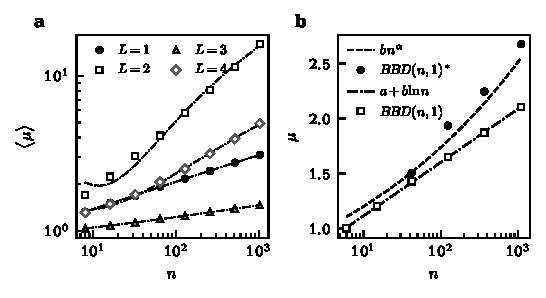
\includegraphics[width=\linewidth]{figs/fig-mu-bubble.pdf}
\caption{\textbf{Cycle length and randomness.} (a) The bubble model $BB(n,L)$,
which closes loops of length $L+2$. Even $L$ (2 and 4) reaches a higher
multiplicity than odd $L$ (1 and 3), as the square-counting predicts --- yet every
$L$ stays log-quadratic, so cycle geometry alone does not buy the exponential.
(b) The deterministic bubble model $BBD(n,1)$ grows only logarithmically, falling
\emph{below} its own randomized version $BBD(n,1)^*$, which follows the power law
of Eq.~\eqref{eq:path-power} with $\alpha\approx0.16$. Locality without randomness
is not enough.}
\label{fig:mu-bubble}
\end{figure}

\section{How fast could it possibly grow?}

If randomness and locality together drive the multiplicity up, it is fair to ask
where the ceiling is. There is one construction for which the question can be
answered exactly, and it is a close relative of the bubble rule: the \emph{diamond
lattice} \citep{migdal1975,kadanoff1976}. Start with a single link joining two
poles $A$ and $B$. At each generation, replace \emph{every} link by two parallel
paths of two links each (Figure~\ref{fig:mu-diamond}a). Where the bubble model
drops one bubble on one randomly chosen link, the diamond drops a bubble on all
links at once, in perfect symmetry.

\begin{calculation}{the multiplicity of the diamond lattice}
The construction is exactly renormalizable, because distinct copies of the
previous generation meet only at their corners. Read it backwards: generation
$G_t$ is two parallel branches, each made of two copies of $G_{t-1}$ in series.
Along a series, lengths add and multiplicities \emph{multiply}; across parallel
branches of equal length, multiplicities \emph{add}. So the pole-to-pole distance
$D_t$ and multiplicity $P_t$ obey
\begin{equation}
  D_t = 2 D_{t-1} = 2^t, \qquad P_t = 2 P_{t-1}^{\,2},
  \label{eq:diamond-rec}
\end{equation}
with $P_0=1$. Taking a logarithm linearizes the recursion and gives
\begin{equation}
  P_t = 2^{\,2^t-1} = 2^{\,D_t-1},
  \label{eq:diamond-pole}
\end{equation}
a \emph{doubly} exponential count. The reason is transparent: a shortest route
must thread $D_t$ successive scales, and at each one it independently picks one of
two parallel branches, so the choices multiply. Averaging over all pairs rather
than the poles alone changes only the prefactor, $\langle\mu\rangle_t \approx
2.1\,P_t/n_t$, since the sum is dominated by near-antipodal pairs. Finally, the
generation carries $n_t = (2\cdot4^t+4)/3$ nodes, so $2^t \simeq \sqrt{3n/2}$, and
substituting into Eq.~\eqref{eq:diamond-pole} turns the doubly exponential in $t$
into a \emph{stretched exponential} in $n$:
\begin{equation}
  \langle\mu\rangle \approx a\,e^{\,b\sqrt{n}},
  \qquad b = \sqrt{\tfrac32}\,\ln 2 \approx 0.849 .
  \label{eq:diamond-n}
\end{equation}
\end{calculation}

The numbers are worth seeing, because they are exact rather than fitted
(Figure~\ref{fig:mu-diamond}b). By the sixth generation the diamond has only
$2732$ nodes, yet an average pair is joined by some $7\times10^{15}$ distinct
shortest paths. This is the fastest growth found anywhere in this chapter, and its
origin is the same parallel branching that the local rules exploit --- only here
it is applied everywhere, at every scale, without a single random choice. Perfect,
maximally symmetric branching therefore sets a hard ceiling on the redundancy a
growing network can carry, and the stochastic local rules of the previous sections
all fall below it.

\begin{figure}[t]
\centering
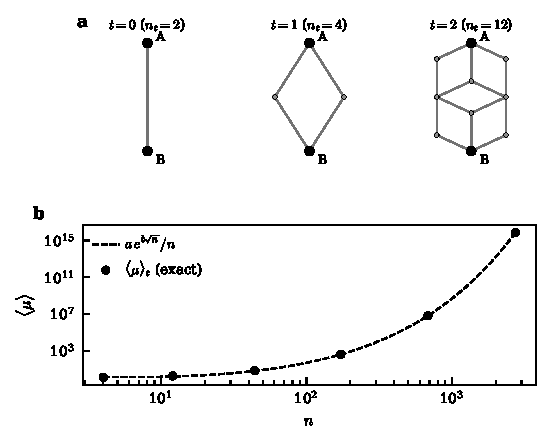
\includegraphics[width=\linewidth]{figs/fig-mu-diamond.pdf}
\caption{\textbf{The exactly solvable ceiling.} (a) The diamond lattice: every
link is replaced, at every generation, by two parallel two-link paths. (b) Its
average multiplicity, computed exactly, follows the stretched exponential of
Eq.~\eqref{eq:diamond-n} across fifteen decades. With $2732$ nodes, a typical pair
of nodes is already joined by some $7\times10^{15}$ equally short routes.}
\label{fig:mu-diamond}
\end{figure}

\section{Two sides of one coin}

Because local rules also create communities, and the number of communities grows
along with the network, we can ask how the multiplicity depends on the number of
communities directly. The relationship is a clean one
(Figure~\ref{fig:mu-local}b and d): linear for every local model tested, and ---
once again the exception --- exponential for duplication--split. This is the
empirical correlation of \citet{deng2026} restated from the inside: more
communities go hand in hand with more shortest paths.

But the point of the chapter is that this partnership is not a case of one
causing the other. ``Local rules boost shortest path multiplicity'' and
``communities accompany high shortest path multiplicity'' are two true statements
about the same networks, and as descriptions they say the same thing. Only one of
them, however, names a \emph{mechanism}. Communities are something an algorithm
reads off a finished network after the fact; the local rule is the process that
actually built that network, node by node, closing the very loops that both carve
it into communities and thread it with redundant routes. Community structure and
path multiplicity are two sides of a single coin --- and the coin is locality.

\section{Real networks}

Models are one thing; the networks we started from are another. Three systems can
be caught at different stages of their growth, which is what we need if we are to
watch $\langle\mu\rangle$ move with $n$ (Figure~\ref{fig:mu-real}). The Internet
at the level of autonomous systems, mapped daily over several years
\citep{snapnets}. The protein interaction networks of a dozen organisms
\citep{stark2006}, which stand in for successive stages of evolution. And the
co-authorship network of the \texttt{cond-mat} preprint archive
\citep{cornellarxiv}, accumulated year by year. In each case we can also compute
the excess degree $c_2$ and so plot the mean-field expectation
$c_2/e$ alongside the measurement --- the random network with the same degrees.
The data are noisy and the systems are not stationary, so no strong claim is
available; but the trends are instructive.

In every system the multiplicity rises with size, and in every system it is
high: the human protein network reaches $\langle\mu\rangle\approx64$, meaning a
typical pair of proteins is joined by some sixty-four equally short chains of
interaction. The protein networks are also the ones that climb
\emph{exponentially} with size, which is the signature of duplication --- and gene
duplication is, of course, exactly how they are thought to grow
(Chapter~\ref{ch:duplication}). The Internet and the co-authorship network both
climb as power laws, more sedately.

The most interesting feature, though, is which side of the mean-field line each
system falls on, because the two disagree in a way that lines up with the degree
correlations of Chapter~\ref{ch:introduction}. The Internet sits \emph{below} its
random expectation: it is \emph{disassortative}, its hubs presiding over
peripheries of poorly connected nodes, and such a star-like arrangement gives a
route no alternatives --- everything must pass through the hub. The co-authorship
network sits \emph{above} it: it is \emph{assortative}, its well-connected authors
writing with one another, and a clique of hubs is exactly what furnishes many
equally short ways across. The same reading applies to the protein networks, which
are disassortative and duly fall below the line. Degree correlations, in other
words, modulate the redundancy on top of what the degrees alone would give ---
a suggestion the mean-field calculation, which knows only $c_2$, cannot yet
account for. It is one of the clearer invitations this book leaves open.

\begin{figure}[t]
\centering
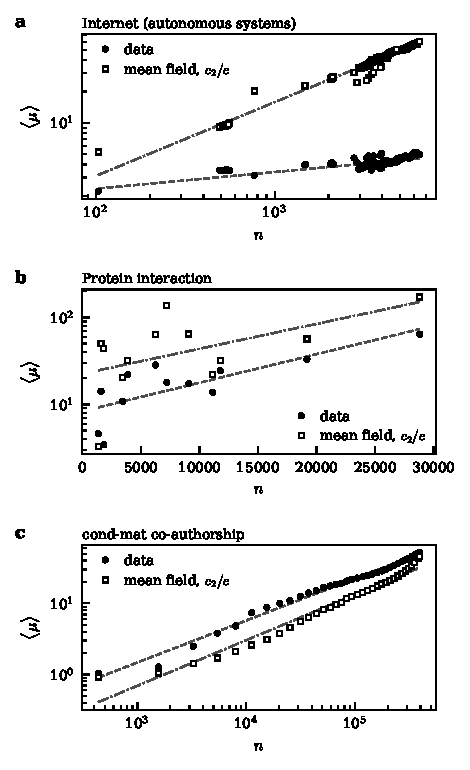
\includegraphics[width=\linewidth]{figs/fig-mu-real.pdf}
\caption{\textbf{Real networks.} Average multiplicity against size, with the
mean-field expectation $c_2/e$ for a random network of the same degrees.
(a) The Internet at the autonomous-system level: a power law, falling below the
random expectation --- the mark of disassortative, star-like wiring. (b) Protein
interaction networks of a dozen organisms: exponential growth, the duplication
signature, reaching $\langle\mu\rangle\approx64$ for the human network. (c)
\texttt{cond-mat} co-authorship: a power law lying \emph{above} the random
expectation, as assortative mixing among prolific authors provides many equally
short routes.}
\label{fig:mu-real}
\end{figure}

\section{Summary}

The shortest paths of real networks are richly redundant, and that redundancy
travels with their community structure. For a random network the redundancy is no
mystery: it is the branching factor, $\langle\mu\rangle\approx c_2/e$, and it
grows only as fast as the hubs allow --- not at all when $\gamma>3$,
logarithmically at $\gamma=3$, as a power law below it. Networks built by local
rules leave that baseline behind, log-quadratically for most rules and
exponentially for duplication, which closes the four-cycles that give opposite
corners two shortest routes apiece. Neither cycle geometry nor locality is
sufficient by itself: a deterministic rule that closes loops everywhere at once
does worse than chance, while the perfectly symmetric diamond lattice, where the
branching can be solved exactly, marks the ceiling at a stretched exponential.
Since the same local rules also produce the communities, the observed tie between
path multiplicity and communities is best understood not as cause and effect but
as two consequences of one underlying local dynamics.
